\documentclass{MScthesisITEM}

% this package is just to generate text for demo-purposes
\usepackage{blindtext}

% Quotes
\usepackage[]{csquotes}
% Todo notes
\usepackage[draft]{todonotes}

\title{Development of an Intelligent Transportation System Testbed} % The title of your assignement; NB use \newlinetitle to start a newline
\author{Ole Andreas Hansen} % Your firstname and lastname
\professor{Wantanee Lastname, ITEM} % Affiliation = ITEM for instance
%\supervisor{Firstname Lastname, Affiliation}

%% Uncomment the following in case you want subfigures; note that there will be a warning for the caption package
% \let\subcaption\undefined
% \let\subfloat\undefined
% \usepackage[bf]{caption}
% \usepackage{subcaption}

\DeclareGraphicsExtensions{.pdf,.jpg}
\graphicspath{{./figs/}}

\loadglsentries{glossary}
\makeglossaries

\begin{document}
\selectlanguage{english}
\pagenumbering{roman}
\pagestyle{plain}

%% Only for the project; comment out the line below for the master's thesis; the front page will be generated automatically by DAIM
\titleITEM

%% Only for the master's thesis; for the project report the description is taken from It's Learning and added by the department
% \selectlanguage{english} % Change to 'norsk' if you are writing in Norwegian
% \begin{titlingpage}

\noindent
\begin{tabular}{@{}p{4cm}l}
\textbf{Title:} 	& \thetitle \\
\textbf{Student:}	& \theauthor \\
\end{tabular}

\vspace{4ex}
\noindent\textbf{Problem description:}
\vspace{2ex}

\noindent \Blindtext[2][1]
\vspace{6ex}

\noindent
\begin{tabular}{@{}p{4cm}l}
\textbf{Responsible professor:} 	& \theprofessor \\
\textbf{Supervisor:}			& \thesupervisor \\
\end{tabular}

\end{titlingpage}
% \cleardoublepage

%% There must be an abstract in English, even though the main text is in Norwegian
\selectlanguage{english}
\pagestyle{empty}
\begin{abstract}
\noindent \Blindtext[5][1]
\end{abstract}
\cleardoublepage

%% Only for the master's thesis; if the main text is in English and you can write Norwegian, there must be an abstract in Norwegian as well.
% \selectlanguage{norsk}
% \pagestyle{empty}
\renewcommand{\abstractname}{Sammendrag}
\begin{abstract}
\noindent Sikkerheten til nesten all offentlig nøkkel-kryptografi er basert på et vanskelig beregnbarhetsproblem. Mest velkjent er problemene med å faktorisere heltall i sine primtallsfaktorer, og å beregne diskrete logaritmer i endelige sykliske grupper. I de to siste tiårene, har det imidlertid dukket opp en rekke andre offentlig nøkkel-systemer, som baserer sin sikkerhet på helt andre type problemer. Et lovende forslag, er å basere sikkerheten på vanskeligheten av å løse store likningsett av flervariable polynomlikninger. En stor utfordring ved å designe slike offentlig nøkkel-systemer, er å integrere en effektiv ``falluke'' (trapdoor) inn i likningssettet. En ny tilnærming til dette problemet ble nylig foreslått av Gligoroski m.f., hvor de benytter konseptet om kvasigruppe-strengtransformasjoner (quasigroup string transformations). I denne masteroppgaven beskriver vi en metodikk for å identifisere sterke og svake nøkler i det nylig foreslåtte multivariable offentlig nøkkel-signatursystemet MQQ-SIG, som er basert på denne idéen.

Vi har gjennomført et stort antall eksperimenter, basert på Gröbner basis angrep, for å klassifisere de ulike parametrene som bestemmer nøklene i MQQ-SIG. Våre funn viser at det er store forskjeller i viktigheten av disse parametrene. Metodikken består i en klassifisering av de forskjellige parametrene i systemet, i tillegg til en innføring av konkrete kriterier for hvilke nøkler som bør velges. Videre, har vi identifisert et unødvendig krav i den originale spesifikasjonen, som krevde at kvasigruppene måtte oppfylle et bestemt kriterie. Ved å fjerne denne betingelsen, kan nøkkel-genererings-algoritmen potensielt øke ytelsen med en stor faktor. Basert på alt dette, foreslår vi en ny og forbedret nøkkel-genereringsalgoritme for MQQ-SIG, som vil generere sterkere nøkler og være mer effektiv enn den originale nøkkel-genereringsalgoritmen.  
\end{abstract}
% \cleardoublepage

\selectlanguage{english}% Change to 'norsk' if you are writing in Norwegian

\renewcommand{\abstractname}{Preface}
\begin{abstract}
\noindent \blindtext 
\end{abstract}
\cleardoublepage

% similarly you may add a separate acknowledgments page

\tableofcontents*
\cleardoublepage

%% include if relevant
\listoffigures
\cleardoublepage

%% include if relevant
\listoftables
\cleardoublepage

%% include if relevant
\listofalgorithms
\addcontentsline{toc}{chapter}{List of Algorithms}
\cleardoublepage

%% include if relevant
\printglossary[title=List of Symbols, style=long]
\cleardoublepage
\glsaddall[]

%% include if relevant
\printglossary[title=List of Acronyms,type=\acronymtype] % prints just the list of acronyms
\cleardoublepage

\pagenumbering{arabic}
\pagestyle{ruled}


%% include here the other chapters
%%
%CHAPTERS
%%
\chapter{Introduction}
\label{chp:introduction} 

\section{Motivation}

\section{Problem Formulation}

\section{Context}

\section{Approach}


\begin{comment}
Here is an example of how to use acronyms such as \gls{ntnu}. The second time only \gls{ntnu} is shown and if there were several you would write \glspl{ntnu}. And here is an example\footnote{A footnote} of citation~\cite{Author:year:XYZ}. 

\Blindtext[3][1]

\begin{figure}
\centering
% dummy figure replacement 
\begin{tabular}{@{}c@{}}
\rule{.5\textwidth}{.5\textwidth} \\
\end{tabular}
\caption{\label{fig:example}A figure}
\end{figure}

\section{First section}\label{sec:first_section}

\subsection{First subsection with some \texorpdfstring{$\mathcal{M}ath$}{Math} symbol}\label{sec:first_ssection}

\blindtext
\begin{itemize}[topsep=-1em,parsep=0em,itemsep=0em] % see http://mirror.ctan.org/macros/latex/contrib/enumitem/enumitem.pdf for details about the parameters
 \item item1
 \item item2
 \item ...
\end{itemize}

\subsection{Mathematics}

\blindmathtrue
\blindtext

\begin{proposition}\label{def:a_proposition}
A proposition... (similar environments include: theorem, corrolary, conjecture, lemma)

\end{proposition}

\begin{proof}
\vspace*{-1em} % Adjust the space when parskip is set to 1em
And its proof.
\end{proof}

\begin{table}
\caption{\label{tab:example}A table}
\centering
\begin{tabular}[b]{| c | c | c | c | c |}
\hline
a & b & c & d & e \\ \hline
f & g & h & i & j \\ \hline
k & l & m & n & o \\ \hline
p & q & r & s & t \\ \hline
u & v & w & x & y \\ \hline
z & æ & ø & å &   \\ \hline
\end{tabular} 
\end{table}

\subsection{Source code example}

% \floatname{algorithm}{Source code} % if you want to rename 'Algorithm' to 'Source code'
\begin{algorithm}[h]
  \caption{The Hello World! program in Java.}
  \label{hello_world}
  % alternatively you may use algorithmic, or lstlisting from the listings package
  \begin{verbatim}
  
class HelloWorldApp {
  public static void main(String[] args) {
    //Display the string
    System.out.println("Hello World!");
  }
}
\end{verbatim}
\end{algorithm}

You can refer to figures using the predefined command like \fref{fig:example}, to pages like \pref{fig:example}, to tables like \tref{tab:example}, to chapters like \Cref{chp:example} and to sections like \Sref{sec:first_section} and you may define similar commands to refer to proposition, algorithms etc.
\end{comment}
\chapter{Background}
\label{chp:Background} 

This chapter explores the area of Intelligent Transportation Systems, its surrounding technologies and the concept of a testbed. Starting with an overview of fundamental concepts in ITS.

\section{Intelligent Transportation System}\label{sec:its}

\blockquote[\cite{eu-10-2010}]{
Intelligent Transport Systems or ITS means systems in which information and communication technologies are applied in the field of road transport, including infrastructure, vehicles and users, and in traffic management ad mobility management, as well as for interfaces with other modes of transport.}

\gls{its} are advanced applications that aims to provide innovative services relating to different modes of transport and traffic management. An \gls{its} service is the provisioning of an \gls{its} application through a well-defined framework with the aim of contributing to user safety, efficiency and comfort. \gls{its} is a part of \gls{iot} that includes \gls{v2v} and \gls{v2i} communication. While the \gls{its} branch i broad this project will mainly focus on the sub-branch Traffic Optimization, which are methods where time stopped in road traffic is reduced. 

\todo[inline]{Go further into EU directives? Penetration of ITS?}

\section{Vehicle-to-Vehicle Communication}\label{sec:v2v}
\gls{v2v} is the ad-hoc networking paradigm and is a vital part of \gls{its}. Vehicular communication systems are networks in which vehicles and roadside units are the communicating nodes, exchanging information with each other such as safety warning, traffic information and location beacons. \gls{v2v} allows car to communicate over the 5.9GHz \gls{dsrc} band. \todo{Quite thin. Maybe more relevant under VANET section?}

%https://www.car-2-car.org/index.php?eID=tx_nawsecuredl&u=0&g=0&t=1518709671&hash=16c41f36747ec4323ca106e60898858277a25dd7&file=fileadmin/downloads/PDFs/MoU_on_deployment-v40001.02_final.pdf
In 2010 a \gls{mou} was signed between the CAR 2 CAR Communication Consortium and multiple car manufactures including Audi, Toyota, BMW, Volvo and Volkswagen among others. The outline of the \gls{mou} is that all car manufactures should commit them self to implement \gls{v2v} in all new cars by 2015. 

\todo[inline]{Include a drawing of V2V communication}

\subsection{Vehicular ad hoc networks}\label{sec:vanet}
Vehicular ad hoc networks (VANETs) uses the principles of mobile ad hoc networks, which is the creation of a wireless network for data exchange, applying this principle to the domain of vehicles. VANETs are a key part of the \gls{its} framework and is used to achieve \gls{v2v} communication and also vehicle-to-infrastructure communication. VANETs can use any wireless networking technology as their basis, such as WLAN, LTE or DSRC. 

\section{Testbed}\label{sec:testbed}
A testbed is a platform for conducting rigorous, transparent and replicable testing of scientific theories, computational tools and new technologies. The term is uses across many disciplines to describe experimental research and new product development platforms and environments. 

\section{Current solutions}
A number of solutions for testing \gls{its} exists and can roughly be divided into two areas: computer simulation and physical tests involving one or more vehicles. Each area with their own pros and cons. 

\subsection{Computer simulations}\label{subsec:computer-simulation}
Computer simulations consists of simulating the environment and different scenarios with software on a computer. Programs such as SUMO and DIVERT is a good starting point for early prototyping and proof of concept for an ITS application. The main drawbacks by simulating on a computer is that it lacks the representation of real world scenarios and variability. Software have a tendency to be too artificial and often gives too optimistic results. But serves as a good baseline for future testing. 

\subsection{Physical testing}\label{subsec:physical-testing}
Physical testing involves testing on real cars in the real world. This type of tests are the best way to test new ITS applications but have some limitations. One major limitation of tests involving vehicles is that outdoor testing can give high costs in terms of logistics and scheduling. Tests have to be performed at a closed location which means that all parties involved need to be transported to the location in order to get started. Another drawback is weather conditions which might not be favorable for the test. As opposed to computer simulation - which are god for initial tests - physical testing is needed when the application is finished with its research stage and moved on to commercialization.

\subsection{Hybrid solution}\label{sec:hybrid-solution}
In this thesis i will try to create a hybrid solution for testing ITS applications. If we can take the best from computer simulation and physical testing, merge those together and create a low-cost, flexible supplement for outdoor testing. 

\subsection{Virtual Traffic Light Testbed}\label{subsec:vtl-testbed}
\todo[inline]{What Anders did}



\chapter{Methodology}
\label{chp:Methodology} 

\section{Introduction}
This chapter serves as the foundation for the implementation phase for this study. It starts with introducing the requirements for the testbed, an introduction to the testbeds hardware and ends with an overview of its characteristics.

\section{Requirements}
The main objective for this project is to create a hybrid solution for testing \gls{its} application taking the advantages from the software simulation models, applying them on low-cost robots and taking the advantages from testing on real cars. In order for this to work we need to fulfill some requirements. Some systems like VANET and GPS needs to be emulated for indoor use. 

\subsection{List of requirements}
\begin{enumerate}
\item \textbf{Flexibility}: Support changes in simulation environment. Different map layouts. Multiple robots

\item \textbf{Communication}: Supplement of VANET/DSRC. Use WiFi. Find some requirements for latency.

\item \textbf{Dynamic Driving}: Cars take independent decisions. Decentralized decision making

\item \textbf{Real-world driving characteristics}: Route planing, speed adaption, awareness

\item \textbf{Localization}: Indoor GPS supplement

\item \textbf{Low Cost}: In order to be feasable 

\end{enumerate}

\section{DiddyBorg V2}
For this project the choice of robots is the DiddyBorg V2 robot which is an upgraded version from the DiddyBorg V1 previously used in Anders Brastad's thesis \cite{DevelopmentOfVTL}. DiddyBorg V2 is a 6 wheeled high-torque robotics platform powered with batteries. It uses six 12V DC gear motors with three mounted on each side of the robot. Its main controlling unit is an on board Raspberry Pi 3 making it highly customizable and suitable for this project. 

\noindent The DiddyBorg robots are one of the most powerful robots available on the market and is easily controlled through a Python API provided by the PiBorg Organization. It can drive over most indoor and outdoor terrain, is able to climb inclines up to 45 degrees and perform a 360 degree turn which makes it suitable for a testbed. Compared to existing solutions for testing \gls{its} application, the simulations can be executed indoor in a controlled environment as opposed to an outdoor test with more variability in its environment. The robots have a low cost - 210 pounds - and are easily customizable and extendable for new use-cases. Figure \ref{fig:diddyborg-robot} shows one of the assembled DiddyBorg robots. 

\begin{figure}[H]
\centering
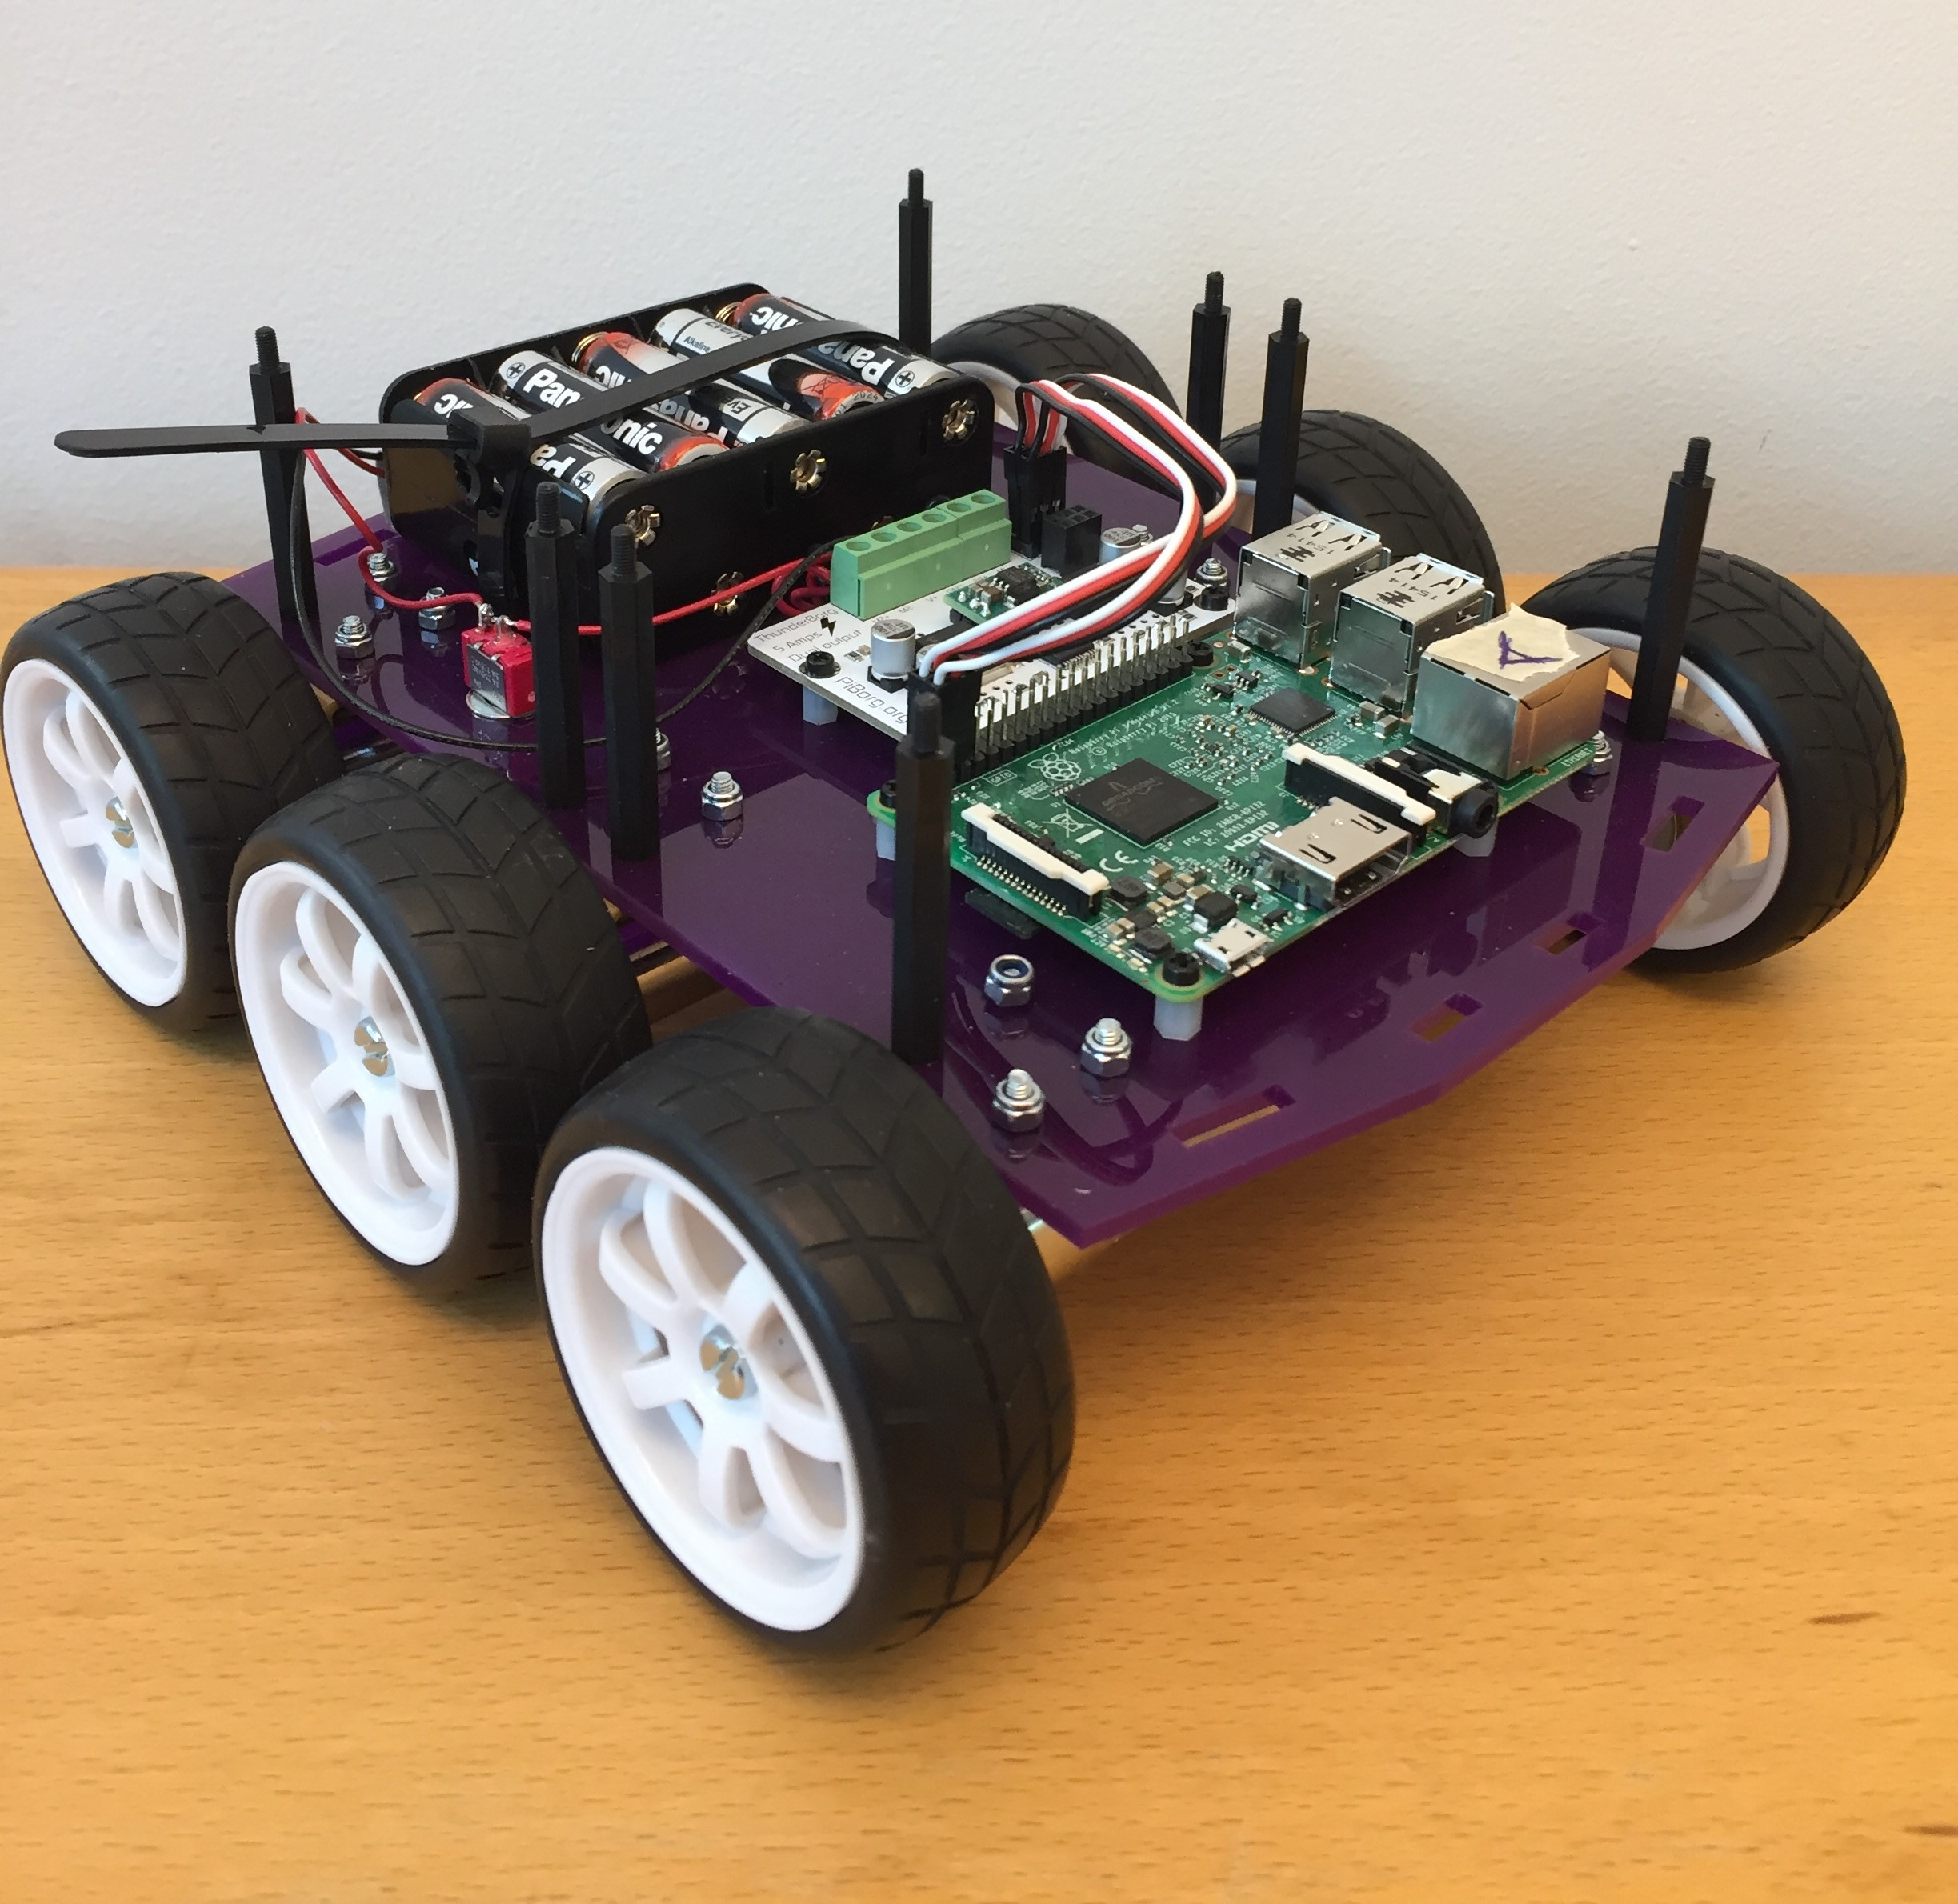
\includegraphics[width=10cm]{images/DiddyBorgV2.jpg}
\caption{Fully assembled DiddyBorg V2 robot}
\label{fig:diddyborg-robot}
\end{figure}

\subsection{Raspberry Pi 3}
Raspberry Pi 3 is a small credit-card-sized computer at a low cost. It can be used as a small personal computer, a media center or as a controlling unit in an electronics project. It comes with a variety of different Operating Systems which is chosen for different types of use. For this thesis the Raspberry Pi is installed with Raspbian as its Operating System. Raspbian is based on Debian and optimized for the Raspberry Pi hardware. It provides an easy to use GUI which makes development and configuration of the unit easier for this project. 

\textbf{Raspberry Pi 3 specifications}
\begin{itemize}
\item Quad Core 1.2GHz 64bit CPU
\item 1GB RAM
\item 4 USB 2 ports
\item Full size HDMI port
\item 40-pin extended GPIO
\item Wireless LAN and Bluetooth Low Energy on board
\item CSI camera port for Raspberry Pi Camera
\end{itemize}

\begin{figure}[H]
\centering
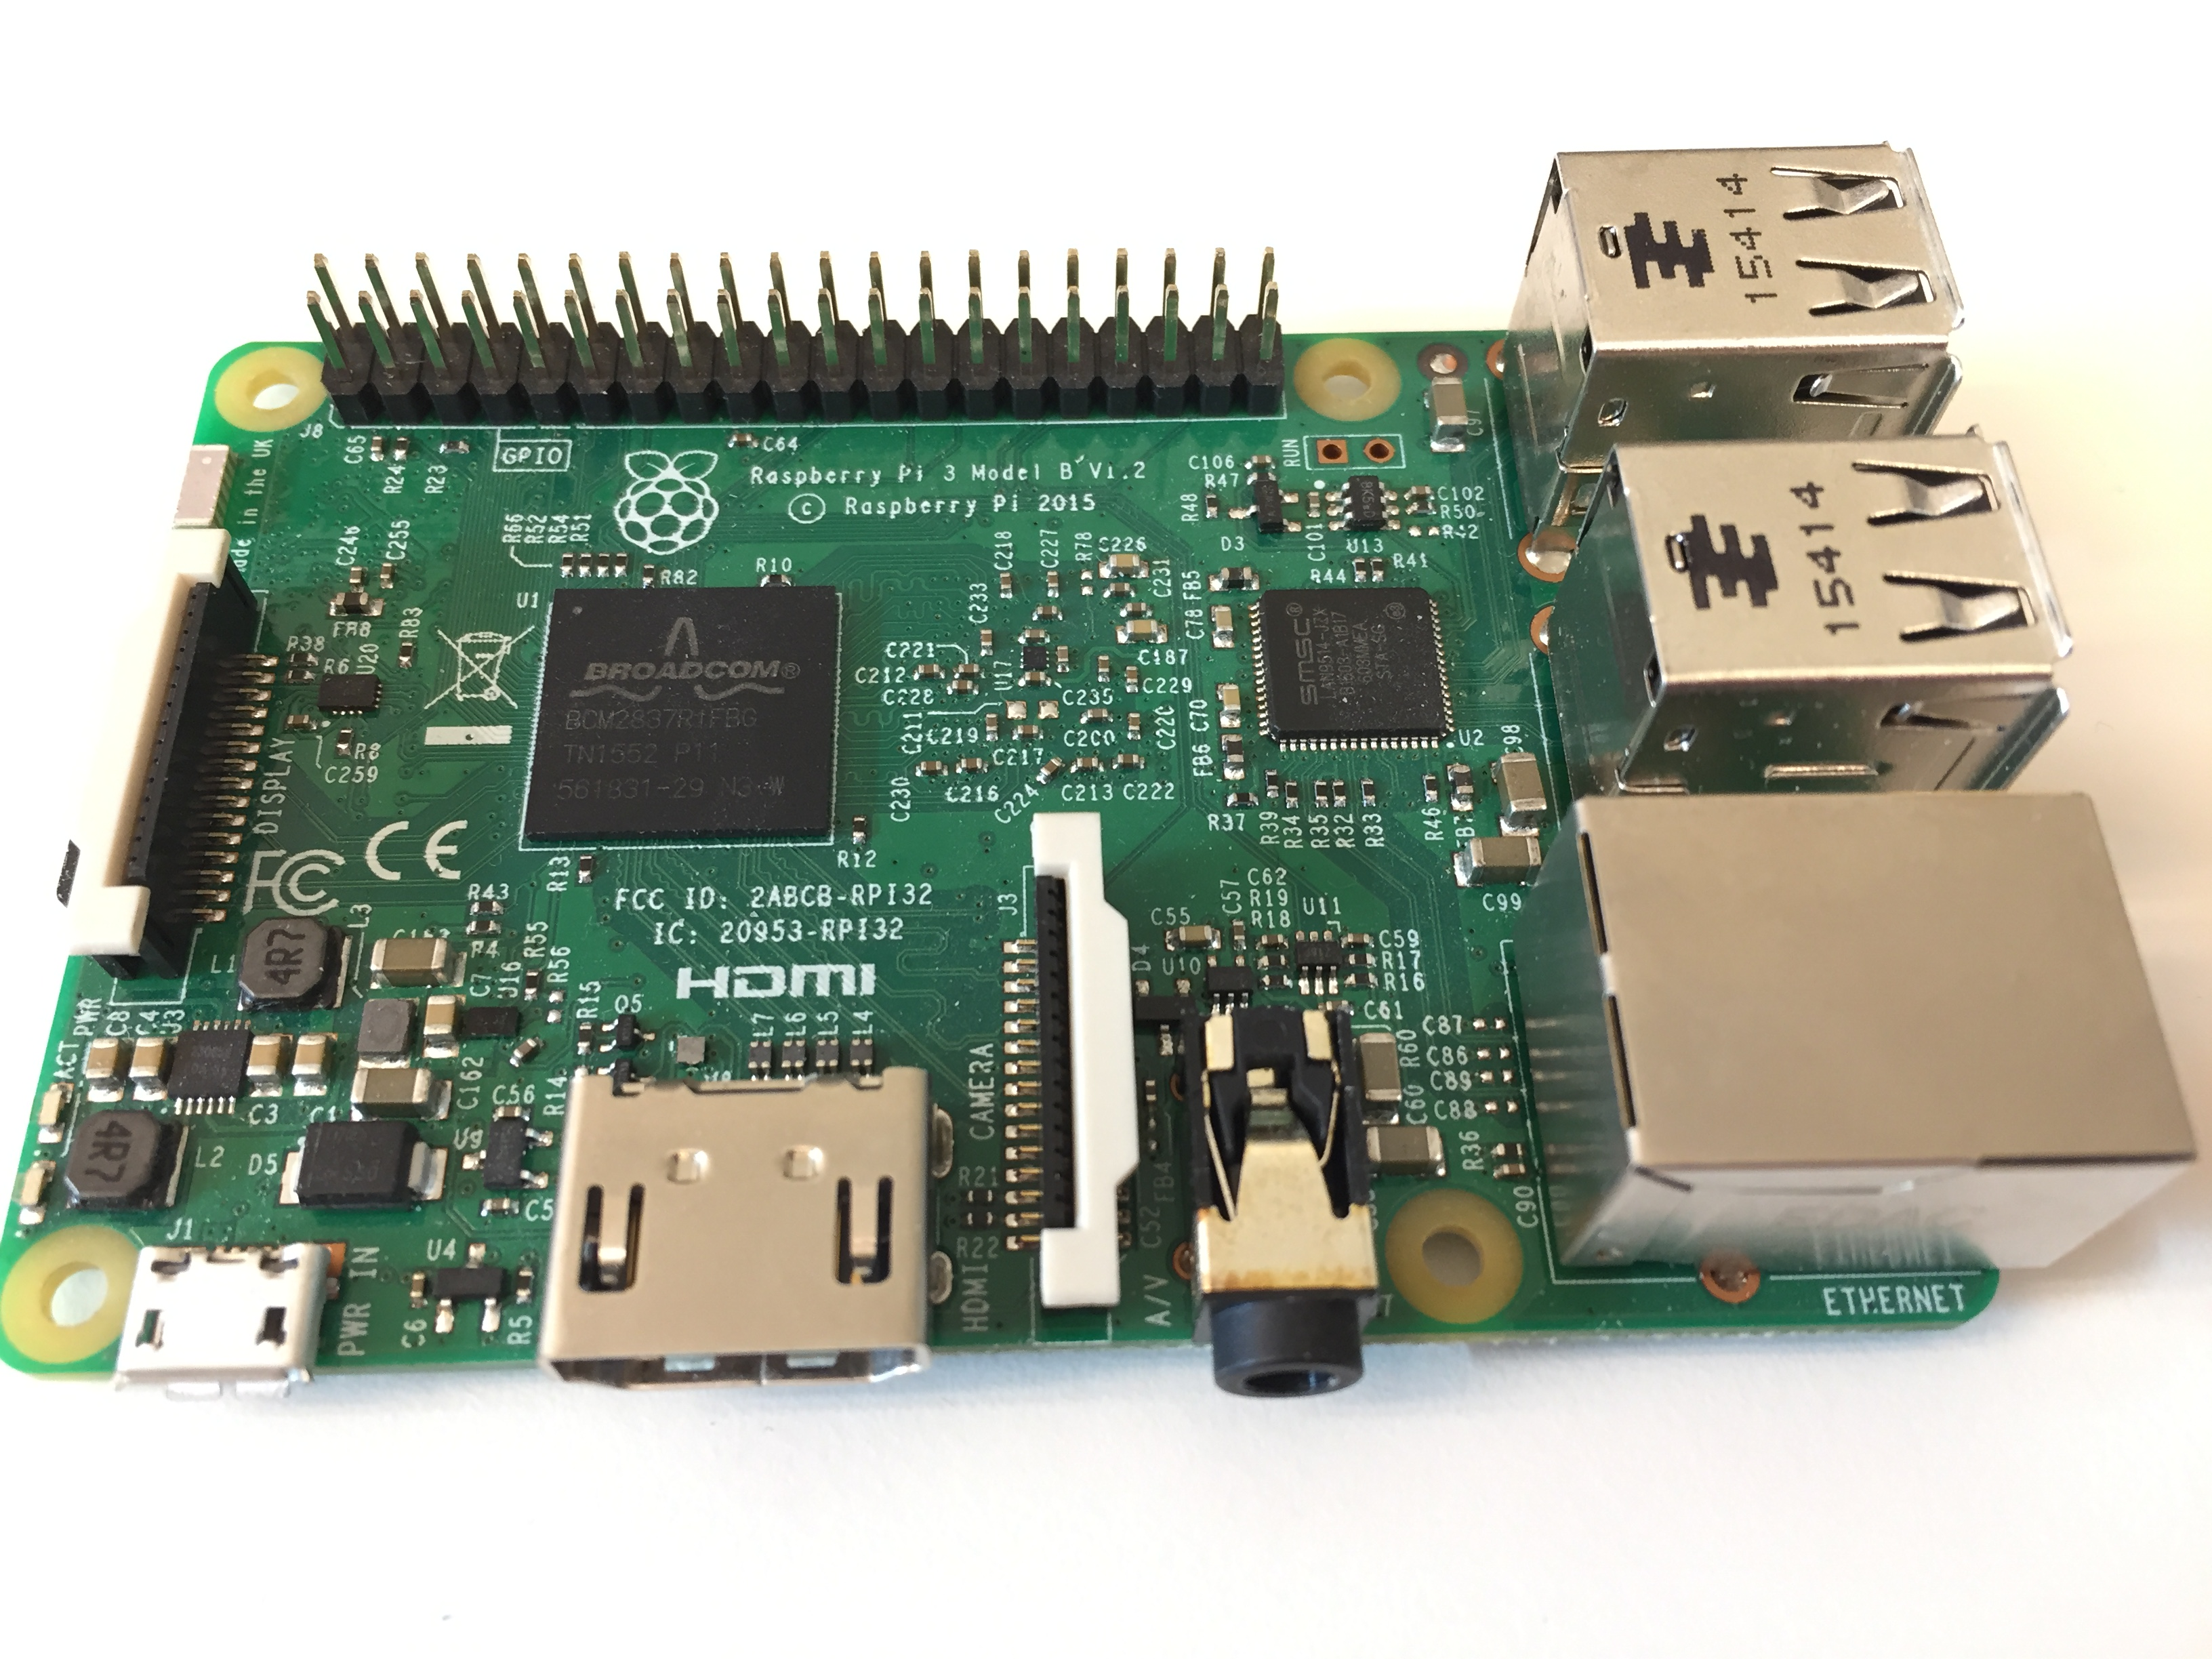
\includegraphics[width=10cm]{images/Raspi3.jpg}
\caption{Raspberry Pi 3}
\label{fig:raspberry-pi}
\end{figure}

\subsection{ThunderBorg}
ThunderBorg is a powerful dual motor control board which makes it possible to power the DiddyBorg motors and the Raspberry Pi with batteries instead of a USB supply. ThunderBorg is directly connected to all six motors and  to the Raspberry Pi via GPIO. The PiBorg organization also provides an easy to use Python API for controlling the motors. A list of available commands are listed in appendix \ref{appendix:thunderborg}. The ThunderBorg board is shown in figure \ref{fig:thunderborg}

\begin{figure}[H]
\centering
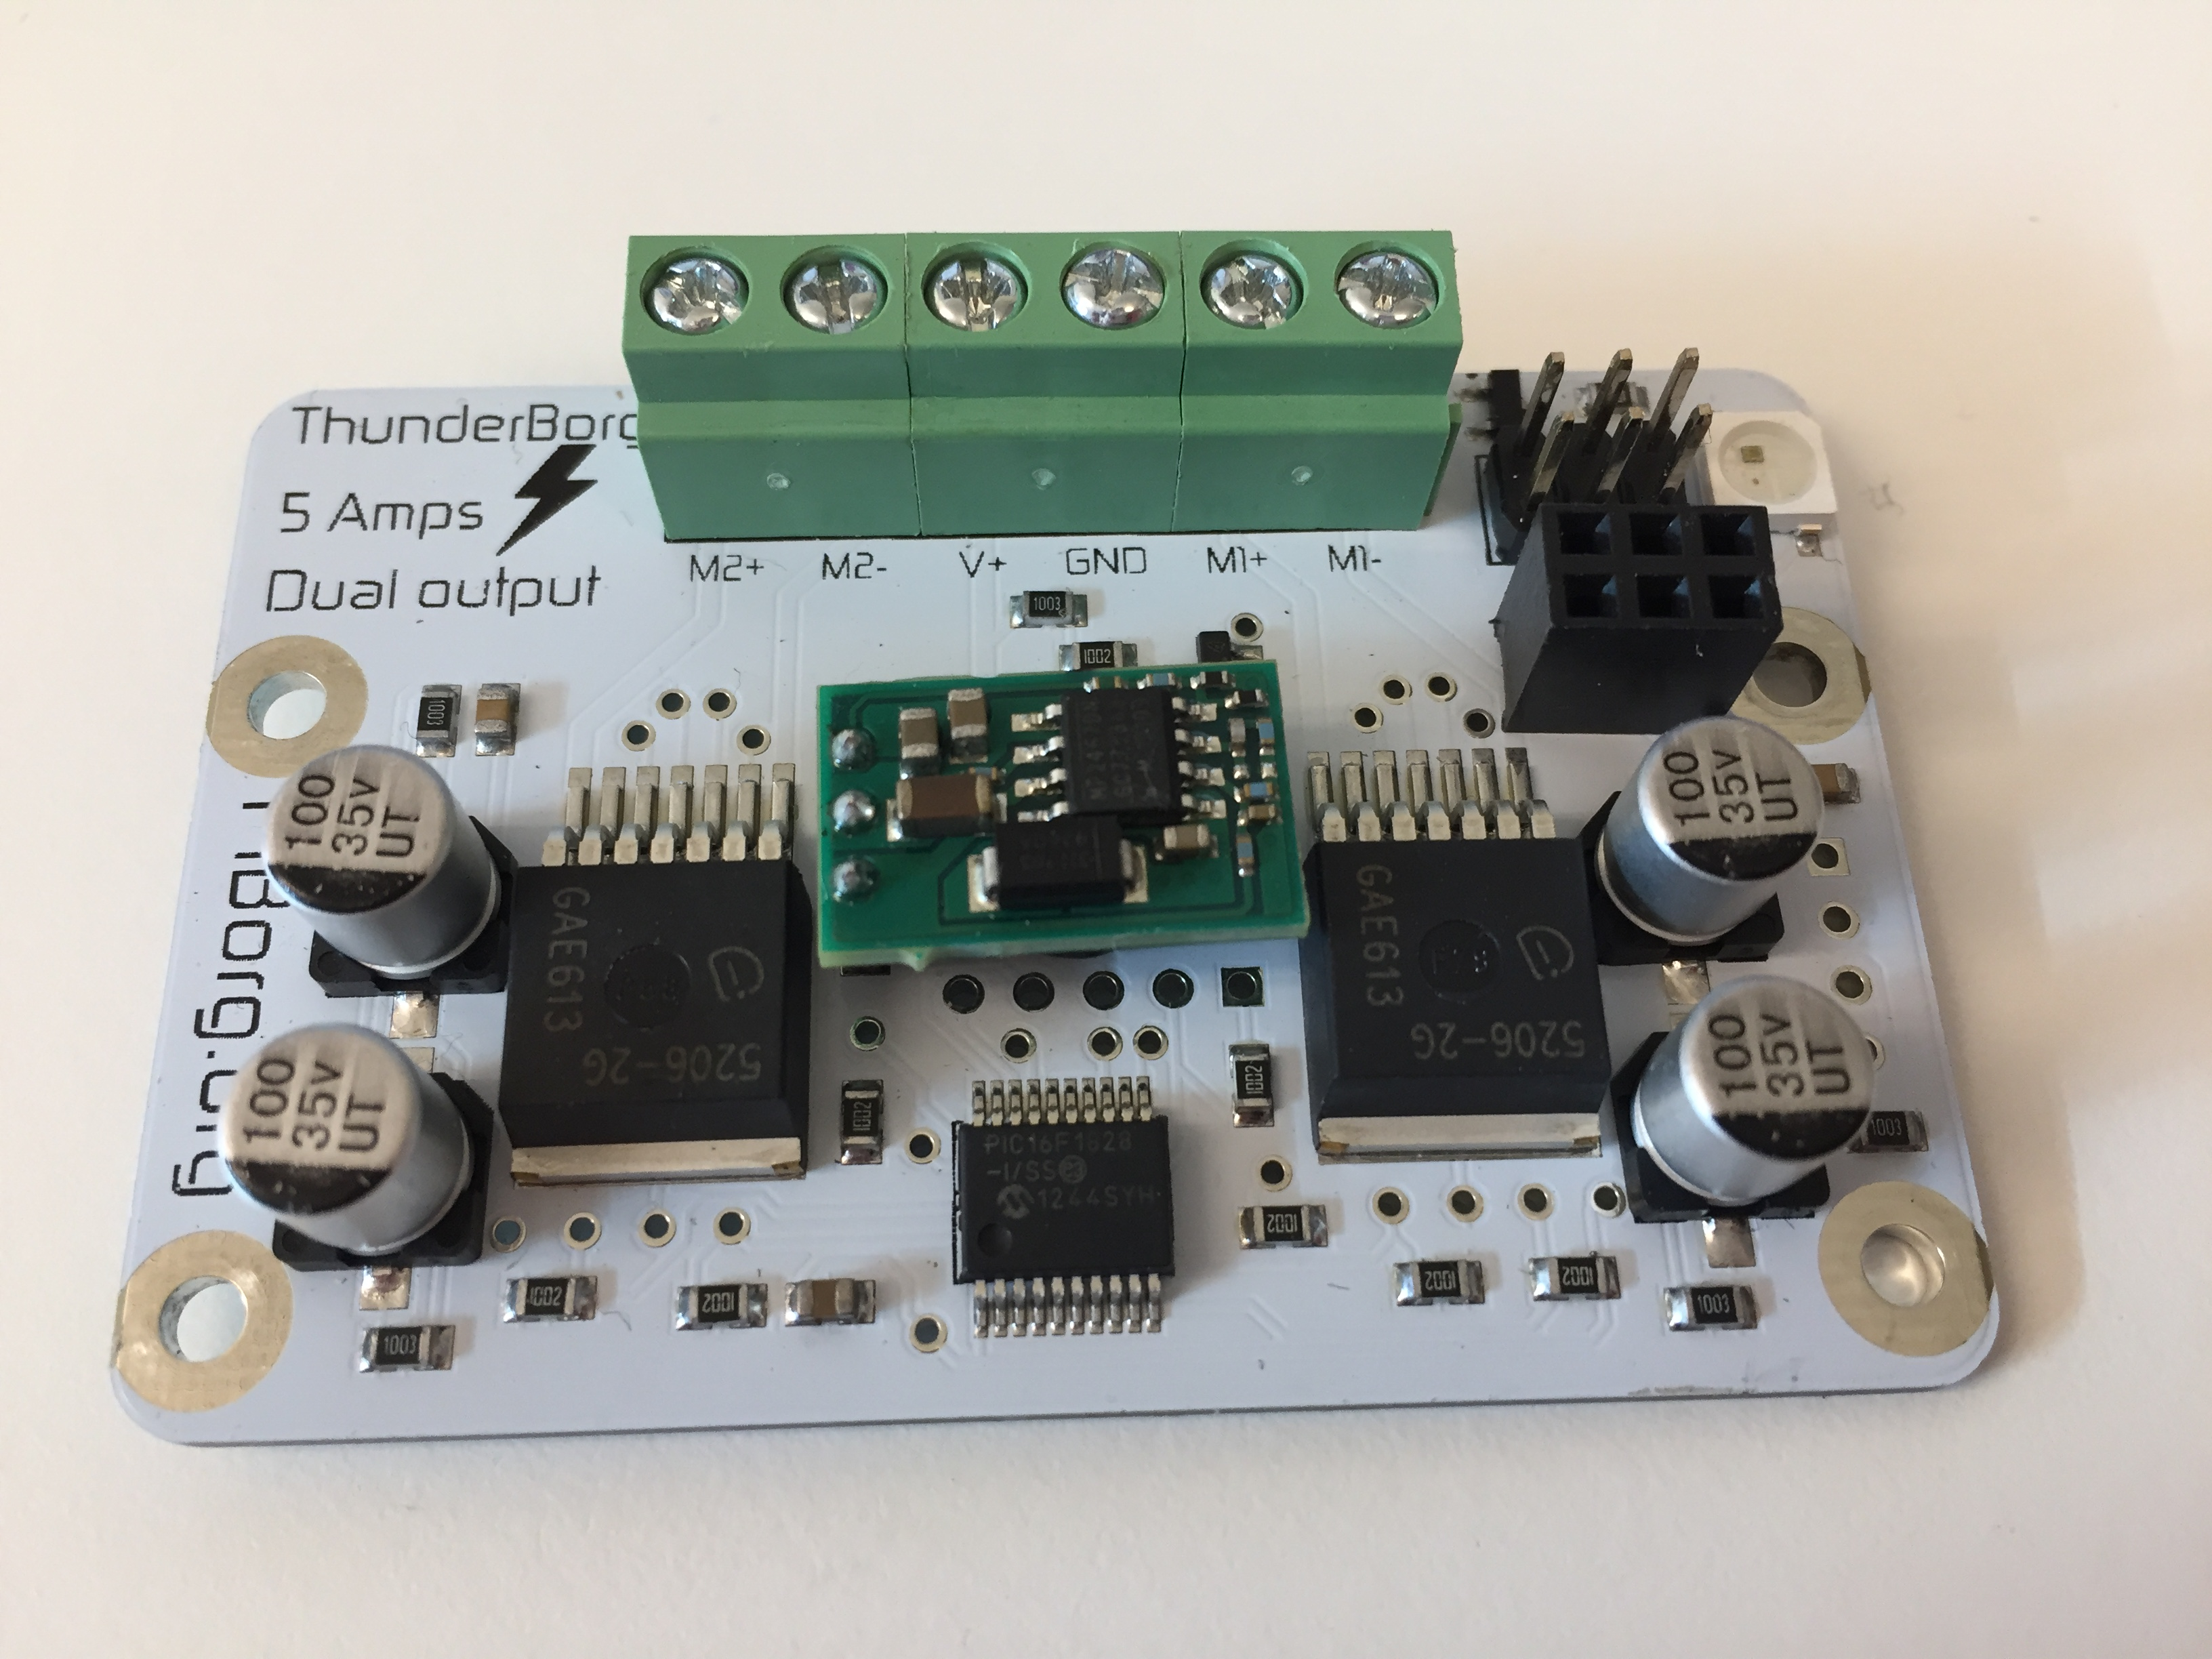
\includegraphics[width=10cm]{images/thunderborg.jpg}
\caption{ThunderBorg}
\label{fig:thunderborg}
\end{figure}

\subsection{Camera}
In order for the robots to have self-driving capabilities they are fitted with a Raspberry Pi Camera. This enables high-definition video for use with image recognition tools such as Lane Detection. The camera is mounted in front of the robot and is used as a solution for indoor localization/positioning. 

\section{Characteristics}
This sections describes some of the key characteristics for the testbed. These characteristics are needed in order to create a base platform to conduct tests and experiments. We need to implement much of the functionality that is and will be available on the market for \gls{its} to be realized in the future. For this project three main characteristics has been selected as the main objectives. 

\subsection{Semi-autonomous driving}
One key component for a traffic optimization testbed is that it needs to support changes in its simulation environment. All robots have an internal map of the surrounding
environment. By allowing this map to be replaced and changed for different simulation scenarios, mechanisms on the robot needs to be implemented. In the
current testbed implementation \cite{DevelopmentOfVTL}, the robots follow a fixed route, driving in a
loop. By allowing changes in environment these fixed routes needs to be dynamic.
\newline
\newline
Another important factor is that the system should simulate actual driving behavior
and support multiple robots. To achieve this multiple mechanisms must be implemented:
map exploration, handling out-of-bounds, indoor positioning, collaboration
between robots and simulation of actual driving behavior. Map exploration and out of bounds is described in section 4.3.

\subsection{Localization}
One key requirement for this projects is to have a system for indoor localization and positioning. For real-world scenarios Global Positioning System (GPS) is the preferred solution that fits the requirements for accuracy and latency. However, a GPS solution does not fit the requirements for this project as it has problems with indoor use and not accurate enough for this project. An indoor positioning system needs to be in place. Implementing a positioning system with software for computer simulations is considered easy and solved. A new problem arises as soon as the system have moving parts which introduces inaccuracy. If the system sends a command to the robot to turn 90 degrees without any confirmation, the robot might over or under turn by some degrees. This inaccuracy will potentially put the robot off course and out of bounds. The system needs to have some kind of component to correct the robots inaccuracy movements. After exploring multiple solutions such as digital compass, ready make indoor positioning system, the choice to use Lane Detection as a correction mechanism was taken. 

\subsubsection{Lane Detection}
Lane Detection is a mechanism used in self-driving cars to detect lanes on roads in real-time. For self-driving cars this method is used to keep the car in the middle of the lanes and to steer in bends. Interestingly, this method can be used as a tool to adjust the robots heading and increase the accuracy of the robots position with respect to the system. \cite{aziz_implementation_2017}

\noindent The process of Lane Detection is as follows:

\begin{enumerate}
    \item Take a frame captured by the Raspberry Pi Camera
    \item Apply an undistortion algorithm to remove camera distortion from the image
    \item Convert the image to gray scale to better separate lanes from roads
    \item Apply some Gaussian smoothing to remove noise on the image
    \item Use an edge detection algorithm (Canny Edge Detection) to detect edges in the image
    \item Trim the image to a region of interest
    \item Apply the Hough Transform algorithms to convert edges on image to physical points/lines in x, y pairs
    \item Apply some linear algebra to create two lines on the image, one for left lane and one for right lane
    \item Average the highest X value on the left lane and the lowest X value on the right lane to get a center point
    \item Compare the current center point to actual center point. If center is higher than actual center, turn slightly left and opposite if the center is lower than actual center
\end{enumerate}

\noindent Figure xx show the output image for each step in the algorithm.

\subsection{Simulate driving behaviour}
In order for the system to represent real-world scenarios it should mock some characteristics that represent normal driving behavior. For this project three key characteristics has been identified. 

\begin{enumerate}
\item \textbf{Route Planning}: Drivers usually drive a partially to fully planned route. This can be achieved by dynamically having a planned route for the robots which also enables a more seamless driving during simulations. 
\item \textbf{Speed Adaption}: When entering and exiting intersections drivers decelerate and accelerate their speed. 
\item \textbf{Consider other cars}: This is important to avoid accidents and to know where other robots are in order to take the correct action.
\end{enumerate}
\chapter{Implementation}
\label{chp:Implementation} 

\section{Introduction}

\section{Architecture}

\section{Planner}

\begin{comment}
- Automated Planning and Scheduling
-- Offline planning: Each car has the whole map, paths can be found prior to execution
- Highest abstraction level
- Goal: Have a path ready for the robot
- Human aspect: We always drive with intention of getting from A to B
- Figure of the planner
- Algorithm
\end{comment}

Planner is the module with the highest abstraction level in the system and its main goal is to provide the cars with some meaning when they are driving. It is responsible for planning a route similar to what humans are doing. Humans are the ones that interact and sends commands to the car. Such as turning the steering wheel, indicating a turn, acceleration etc. The normal objective for a car is to transport people from A to B. The planner takes the job of always having a route for the robot to perform. Self driving cars also have the same objective, the driver tells the car where to go and the car creates a plan for this trip from A to B. 

\noindent For this projects, the environment and world map is quite simplified. There are only straight roads with simple intersections which reduces the complexity of the planner.

% http://www.cambridge.org/no/academic/subjects/computer-science/artificial-intelligence-and-natural-language-processing/automated-planning-and-acting?format=HB&isbn=9781107037274#ItlLzJTDtjPBw6TX.97
\noindent The idea of having a planner is based upon the theory of \gls{aps}, a branch of artificial intelligence that concerns the realization of strategies or actions sequences. For this thesis one of the assumptions is that all robots have a complete internal map of the environment, this means that planning can be performed offline. A solution can be found and evaluated prior to execution. In a real world scenario, in dynamically unknown environments the strategy often needs to be revised online. 

\noindent Given a description of the possible initial states in the world, a description of the desired goals, and a description of a set of possible actions, the planning problem is to synthesize a plan that is guaranteed (when applied to any of the initial states) to generate a state which contains the desired goals - the goal state. 

\noindent The simplest possible planning problem, known as the Classical Planning Problem is determined by:
\begin{itemize}
    \item a unique known initial state
    \item durationless actions
    \item deterministic actions
    \item which can be taken only one at a time
    \item a single agent
\end{itemize}

\noindent Since the initial state is know unambiguously, and all actions are deterministic, the state of the world after any sequence of actions can be accurately predicted, and the question of observability is irrelevant for classical planning. 

\noindent Given the above peculiarities the job of the planner simplifies for this project. In order for the system to guarantee full environment exploration, only a given number of steps or commands are calculated by the planner. We can construct a finite state machine that describes the planner as seen in figure \ref{fig:planner-state-machine}

\begin{figure}[H]
\centering
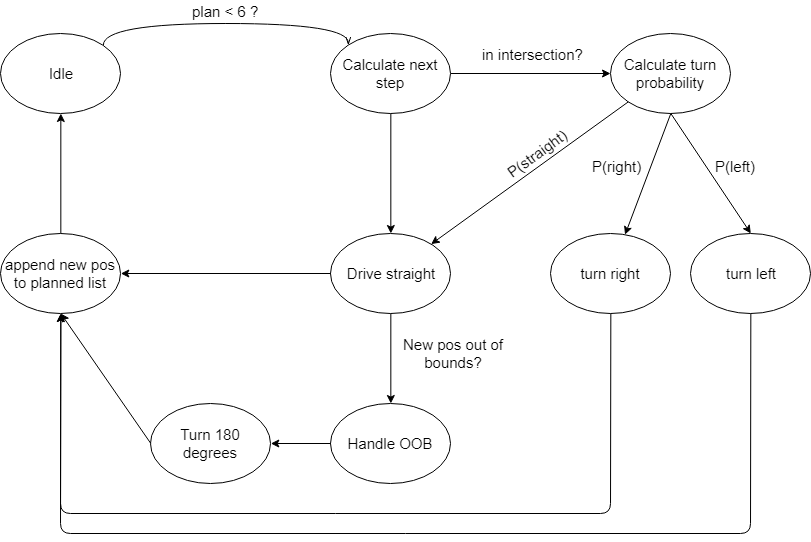
\includegraphics[width=10cm]{figs/Planner-State-Machine.png}
\caption{Planner Finite State Machine}
\label{fig:planner-state-machine}
\end{figure}

\noindent The basic operation of the planner is shown in algorithm \ref{algo:planner} in a simplified manner. The full implementation of the planner module is found in appendix X. 

\begin{algorithm}[ht]
    \caption{Basic operation for the planner module}
    \label{algo:planner}
    \begin{algorithmic}
    \While {thread is active}
        \If {$queue\_length < max\_plan\_size:$}
            \If {current location not in intersection}
                \State Add drive straight to plan
            \Else
                \State $probability = random\_probability$
                \If {$probability$ < probability of turning left}
                    \State Add turn left to plan
                \ElsIf {$probability$ < probability of turning right}
                    \State Add turn right to plan
                \Else
                    \State Drive straight
                \EndIf
            \EndIf
        \EndIf
    \EndWhile
    \end{algorithmic}
\end{algorithm}

\noindent The planner module is instantiated/initiated by the car module. Before any movement takes place the planner creates a list of 6 commands which serves as the path/plan for the robot to perform. Each time the robot is to perform a move the first command in the planner list is removed and its appropriate action is calculated based on the command. As depicted in figure \ref{fig:planner-state-machine} there are four possible actions created by the planner: drive straight, turn left, turn right and turn 180\textdegree. These commands are interpreted and consumed by the car module described in section \ref{sec:car-module}.

\section{Network}
One central aspect in order to have a working testbed is the network. In this thesis the network topology and the network module together serves as the replacement for \gls{vanet} and \gls{dsrc}. MENTION WLAN. The following subsections describe the network topology (VANET) and the onboard network module (DSRC) that provides communication. 

Raspberry Pi 3 comes with an onboard wireless interface which will serve as the \gls{dsrc} device for the robots

\subsection{Network Topology}
Raspberry Pi 3 comes with an onboard wireless interface that is used to send and receive packets in this project. Preferably, the setup of this interface should utilize the ad-hoc functionality provided by 802.11n. Due to problems of making this functionality work as expected, the ad-hoc functionality has been disabled in order to have a reliable system. 

In order for this communication to work, some configuration needs to be done on the Raspberry Pi. This is done by editing the network interface file located at $/etc/network/interfaces$. Figure \ref{fig:network-settings} displays the network configuration settings used on all Raspberry Pis in this thesis.

\begin{figure}
    \centering
    \begin{verbatim}
        auto wlan0
        iface wlan0 inet static
            address 192.168.1.1 # This address has to be unique
            netmask 255.255.255.0
            wireless-channel 1
            wireless-essid its_testbed
            wireless-mode ad-hoc
    \end{verbatim}
    \caption{\label{fig:network-settings}Network settings on Raspberry Pi}
\end{figure}

When configuring all devices in our testbed with the same settings, assigning each Raspberry Pi with a unique static IP-address, er can communicate on a peer-to-peer basis or \gls{v2v} in an ad-hoc manner. Notably, this enables the devices to communicate with every device in its vicinity. Figure \ref{fig:raspi-ad-hoc} shows the topology of the ad-hoc network in this project.

\begin{figure}
\centering
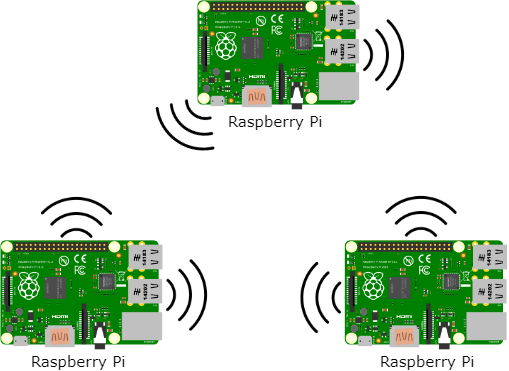
\includegraphics[width=10cm]{figs/raspi-ad-hoc.png}
\caption{Ad hoc network with Raspberry Pi 3 devices}
\label{fig:raspi-ad-hoc}
\end{figure}

\subsection{Network Module}
The network module is the module responsible for crafting, sending and receiving packets to and from other robots. For this project this module acts as the DSRC device or Onboard Unit (OU) of the car. This module is separated into two logical parts: one for sending messages and one for receiving messages, where they provide different functionality to the system. 

The concepts of \gls{vanet} and \gls{vtl} requires the use of broadcast messages in the network in order to exchange beacons (as described in...). There is also a need to separate the types of messages sent. In this projects there are two available message types: one for periodically sending beacons and one that is application specific. Since this testbed is to be a general purpose testbed for \gls{its} applications and implementation of application specific messages needs to be developed to fit the \gls{its} application being tested. In this project, an example implementation has been done for a centralized regular traffic light and a decentralized implementation of the \gls{vtl} algorithm as described in (A distributed Algorithm for VTL with IEEE 802.11p). The code for these implementations can be found in appendix X and Y. 

To handle this, the Python socket module is used. With this, one can bind a socket to an IP-address and port for sending and receiving packets over the network. In this setup User Datagram Protocol (UDP) is used for sending messages. Another option is to use the TCP protocol but this requires more overhead in the system. There are no guarantee that a UDP packet will reach its destination, which is the same for the current solutions for VANET/DSRC. To make a socket able to broadcast messages to all devices within its vicinity, the socket has to be tied up to the network broadcast address. In this network setup, the broadcast address is $192.168.1.255$. Upon receiving messages from the network, a server socket listening to messages sent to its IP-address and port, is established.

Figure x is a sequence diagram explaining how a broadcast message is sent through the ad-hoc network and received at all connected nodes. Raspberry Pi A is the sender of the message to the broadcast address. A message sent to this address will be delivered to all connected nodes in the range of the source. For the receivers - Raspberry Pi B and C - the message seems to come directly from Raspberry Pi A. 

\begin{figure}
\centering
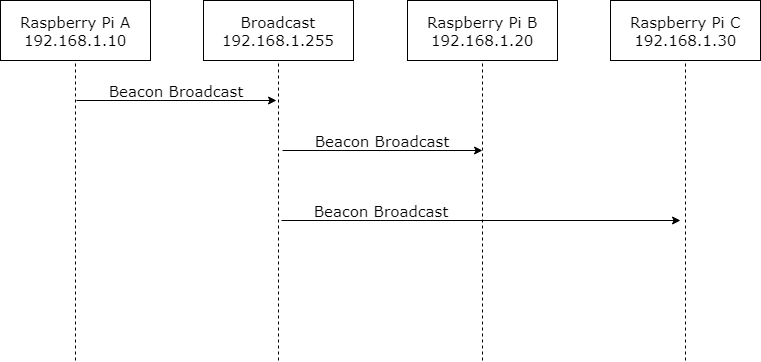
\includegraphics[width=12cm]{figs/Broadcast-Message.png}
\caption{Sequence diagram showing the flow of a broadcast message}
\label{fig:broadcast-message}
\end{figure}

\begin{figure}
\centering
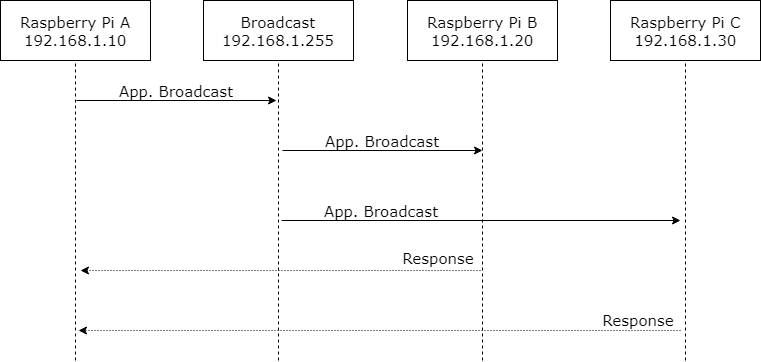
\includegraphics[width=12cm]{figs/App-Specific-Message.png}
\caption{Sequence diagram showing the flow of a application specific message with reply}
\label{fig:app-message}
\end{figure}

\begin{comment}
- VANET / DSRC
- Send / Receive
- Beacons and application specific messages
- Broadcast
\end{comment}

\section{Location}

\subsection{Environment}

\subsection{Lane Detection}

\section{Environment}

\section{Motor Control}

\section{Car}\label{sec:car-module}

\section{Data Flow}

\section{Challenges}
\chapter{Testing}
\label{chp:Testing} 

\section{Initial testbed simulations}

\section{Virtual Traffic Light simulation}

\section{Results}
\chapter{Conclusion}
\label{chp:Conclusion} 

\section{Summary}

\section{Evaluation}

\section{Future work}



\renewcommand*{\bibname}{References}
\bibliographystyle{alpha}
\bibliography{main}

%% Uncomment the following if you have any appendix
\appendix
 \addtocontents{toc}{%
  \protect\vspace{1em}% 
  \protect\noindent \bfseries \appendixtocname\protect\par
  \protect\vspace{-.5em}%
 }
\renewcommand{\chaptername}{\appendixname}
%% include below possible appendices (chapters)
\chapter{Available ThunderBorg commands}
\begin{itemize}
\item \textbf{RawWrite()} Sends a raw command on the I2C bus to the ThunderBorg 
\item \textbf{RawRead()} Reads back from the ThunderBorg after sending a GET command
\item \textbf{InitBusOnly()} Prepare the I2C driver for talking to a ThunderBorg on the specified bus and I2C address.
\item \textbf{Init()} Prepare the I2C driver for talking to the ThunderBorg
\item \textbf{SetMotor2()} Sets the drive level for motor 2, from +1 to -1
\item \textbf{GetMotor2()} Gets the drive level for motor 2, from +1 to -1
\item \textbf{SetMotor1()} Sets the drive level for motor 1, from +1 to -1
\item \textbf{GetMotor1()} Gets the drive level for motor 2, from +1 to -1
\item \textbf{SetMotors()} Sets all motors to stopped, useful when ending a program
\item \textbf{SetCommsFailsafe()} Sets the system to enable of disable the communication failsafe. The failsafe will turn the motors off unless it is commanded at least once every 1/4 of a second.
\item \textbf{GetCommsFailsafe()} Read the current system state of the communications failsafe. 
\item \textbf{GetDriveFault1()} Reads the motor drive fault state for motor \#1. Faults may indicate power problems, such as under-voltage and may be cleared by setting a lower drive power. 
\item \textbf{GetDriveFault2()} Reads the motor drive fault state for motor \#2. Faults may indicate power problems, such as under-voltage and may be cleared by setting a lower drive power. 

\end{itemize}
\label{appendix:thunderborg}

\end{document} 
